\documentclass{article}
\usepackage[brazil]{babel}
\usepackage[utf8]{inputenc}
\usepackage[T1]{fontenc}% optional T1 font encoding
\usepackage[%
    colorlinks=true,
    pdfborder={0 0 0},
    linkcolor=red
]{hyperref}
\usepackage[all]{hypcap}
\usepackage{amsmath}
\interdisplaylinepenalty=2500
\usepackage{graphicx}
\usepackage[cmintegrals]{newtxmath}
\usepackage{cite}
\usepackage{listings}
\usepackage{hyperref}
\usepackage{indentfirst}
\usepackage{siunitx}
\usepackage{textgreek}
\usepackage[portuguese,linesnumbered,ruled]{algorithm2e}
\usepackage{multirow}
\usepackage{anysize}

\begin{document}

    \title{Preparação do Exp. V — Amplificador de áudio classe AB (\emph{push-pull)}}
    \author{Bianca Yoshie Itiroko - 164923, Luiz Eduardo Cartolano - 183012, Seong Eun Kim - 177143 \\ EE534 - Turma Y - Grupo 2}
    \date{Outubro de 2018}

    \maketitle

    \section{Parâmetro do diodo 1N4004}
        Usando o \emph{datasheet} do diodo 1N4004, que pode ser encontrado em \citeonline{ref:datasheet}, foi possível determinar a \emph{forward voltage} do diodo para a corrente de 1A, o valor encontrado foi de $1V$. A simulação pode ser vista em \citeonline{ref:simu}.

    \section{Funcionamento do circuito} \label{sec:1}
        O circuito da Figura \ref{fig:push-pull} é conhecido como \emph{push-pull}, ele é um amplificador de classe AB, e tem como objetivo ser mais eficiente do que os vistos em experimentos anteriores. Ele costuma ser usado onde saída de alta potência elevada e fidelidade são necessárias, como em estágios da saída do receptor, moduladores AM, etc.
        
        Analisando sua simulação, que pode ser vista em \citeonline{ref:simu}, podemos perceber algumas peculiaridades do mesmo. Uma delas é a presença de dois diodos, estes tem a função de manter os transistores continuamente polarizados, e  assim evitar \emph{cross-distortion}. Isso acontece porque os diodos garantem uma tensão entre a base e o emissor dos transistores entre $0,6V$ e $0,7V$.
        
        Uma segunda análise interessante está no funcionamento geral do circuito. Primeiro, é possível perceber que ao colocarmos um valor de $V_{in} = 0V$, não há corrente circulando pelo circuito (vide Figura \ref{fig:vin0}), o que evita dissipação inútil de potência pelos componentes, ou seja, temos um circuito mais eficiente. Além disso, é interessante notar que, ao contrário dos demais experimentos, dessa vez estamos trabalhando com dois transistores de polarização diferente, um de tipo N e outro de tipo P, o que faz com que, ao usar uma fonte de tensão alternada, nosso \emph{output} se mantenha constante independente de estarmos em um semi-ciclo positivo ou negativo de tensão. No semi-ciclo positivo (Figura \ref{fig:push-pull-pos}), o transistor \emph{NPN} estará em funcionamento, enquanto que o transistor \emph{PNP} estará em corte. A situação se inverte no semi-ciclo negativo. O que nos permite concluir que, na verdade, o circuito estudado é composto por dois circuitos \emph{seguidor de emissor} que funcionam de modo complementar, garantindo um ganho de tensão unitário, com aumento da corrente de saída com baixa impedância por um custo menor do que o do \emph{seguidor de emissor}.
 
        
    \nocite{*}
    \bibliographystyle{plain}
    \bibliography{references}

    \begin{figure}[!h]
        \centering
        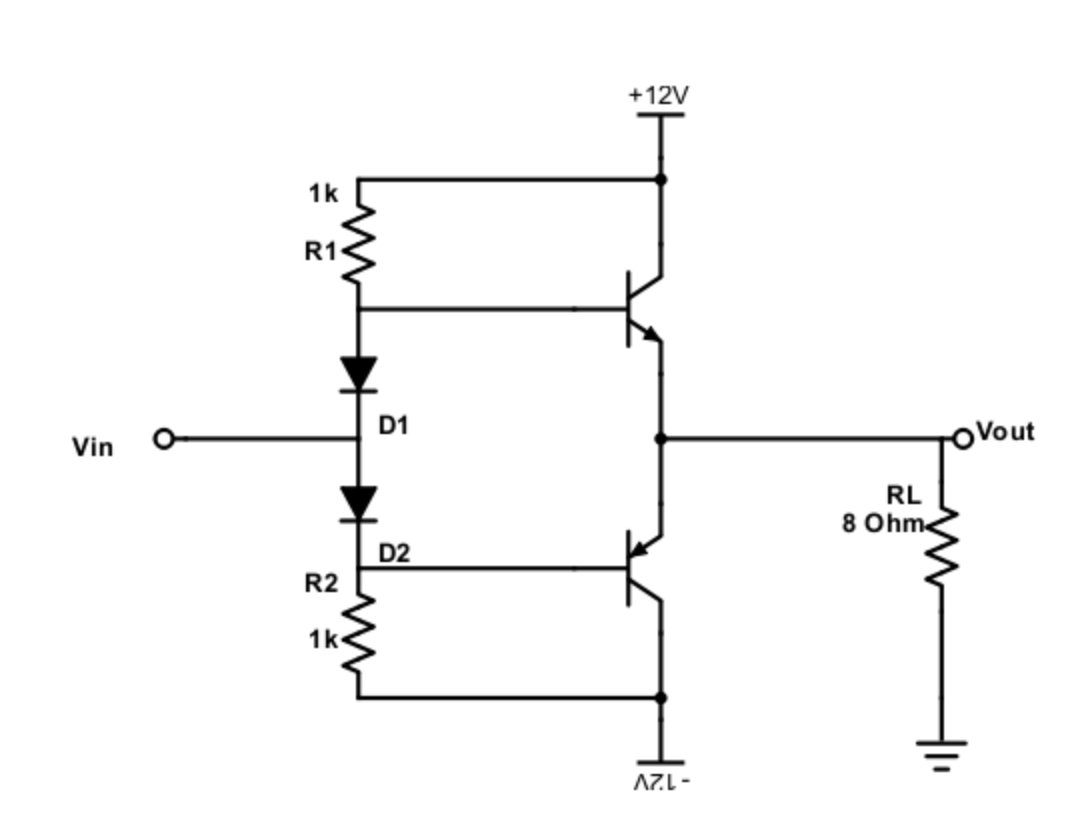
\includegraphics[width=13cm,height=13cm,keepaspectratio]{imagens/circ1.png}
        \caption{Circuito \emph{push-pull}.}
        \label{fig:push-pull}
    \end{figure}

    \begin{figure}[!h]
        \centering
        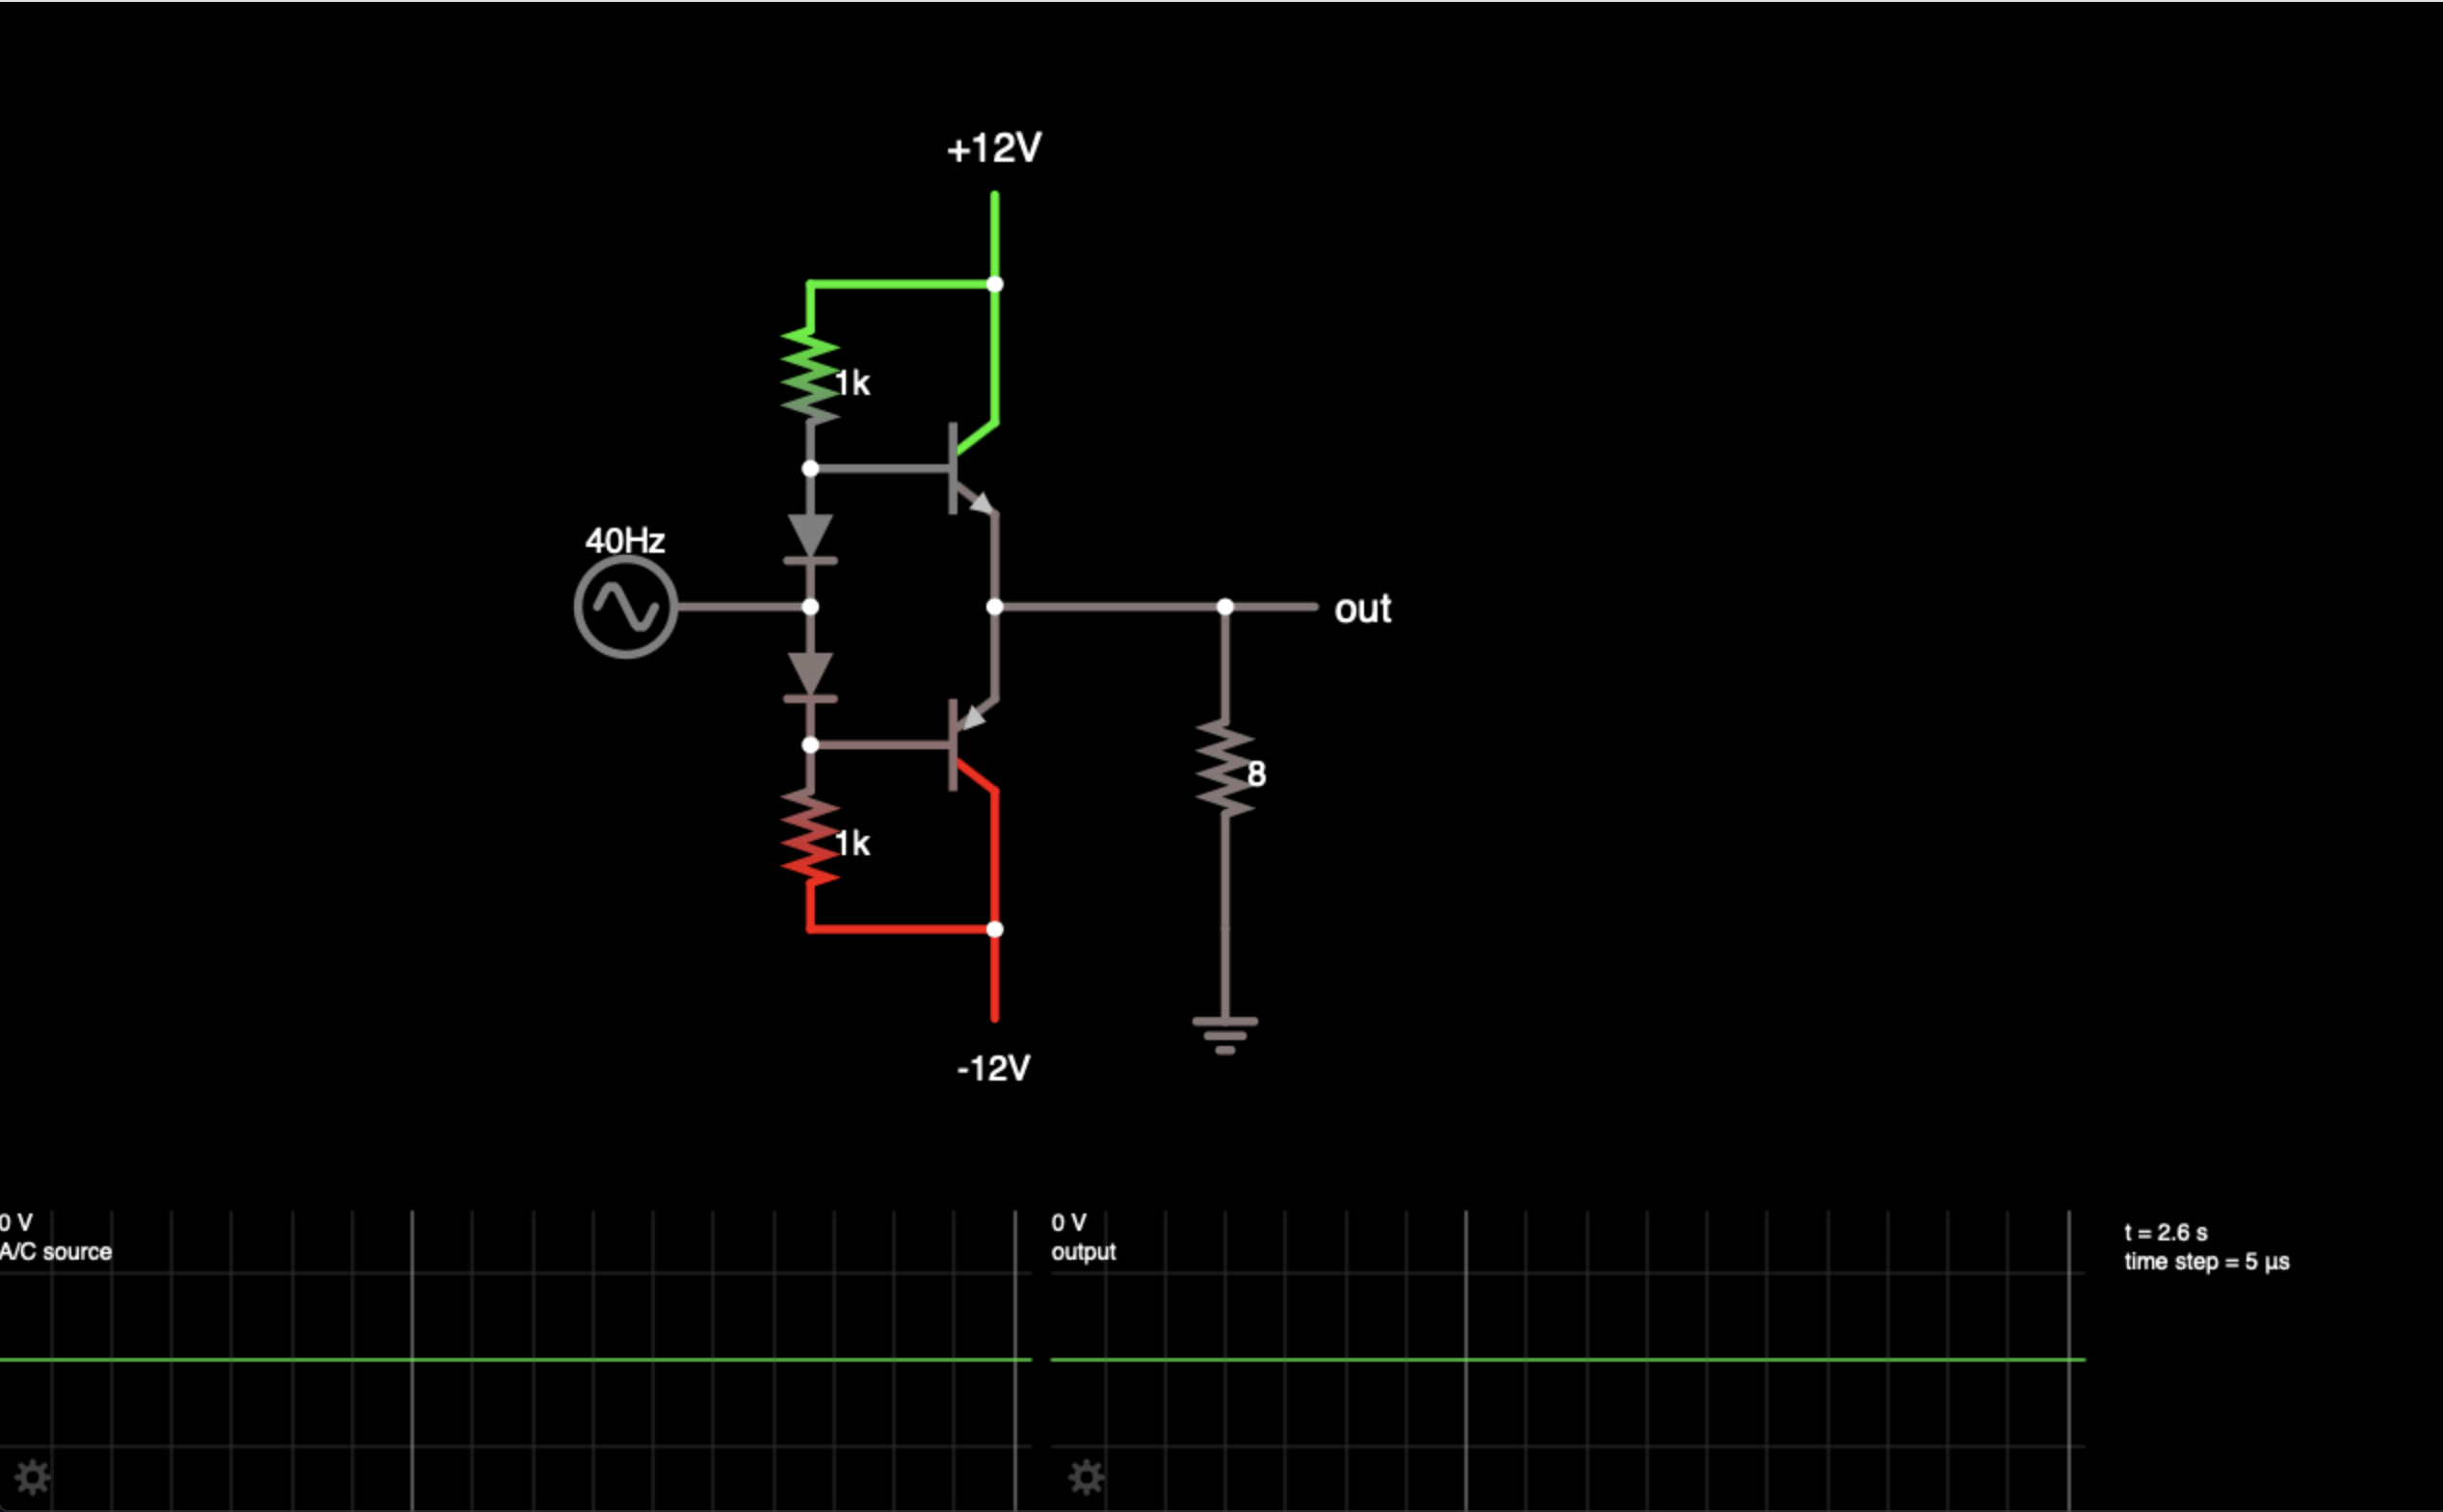
\includegraphics[width=13cm,height=13cm,keepaspectratio]{imagens/vin0.png}
        \caption{Circuito \emph{push-pull} com $V_{in} = 0$.}
        \label{fig:vin0}
    \end{figure}

    \begin{figure}[!h]
        \centering
        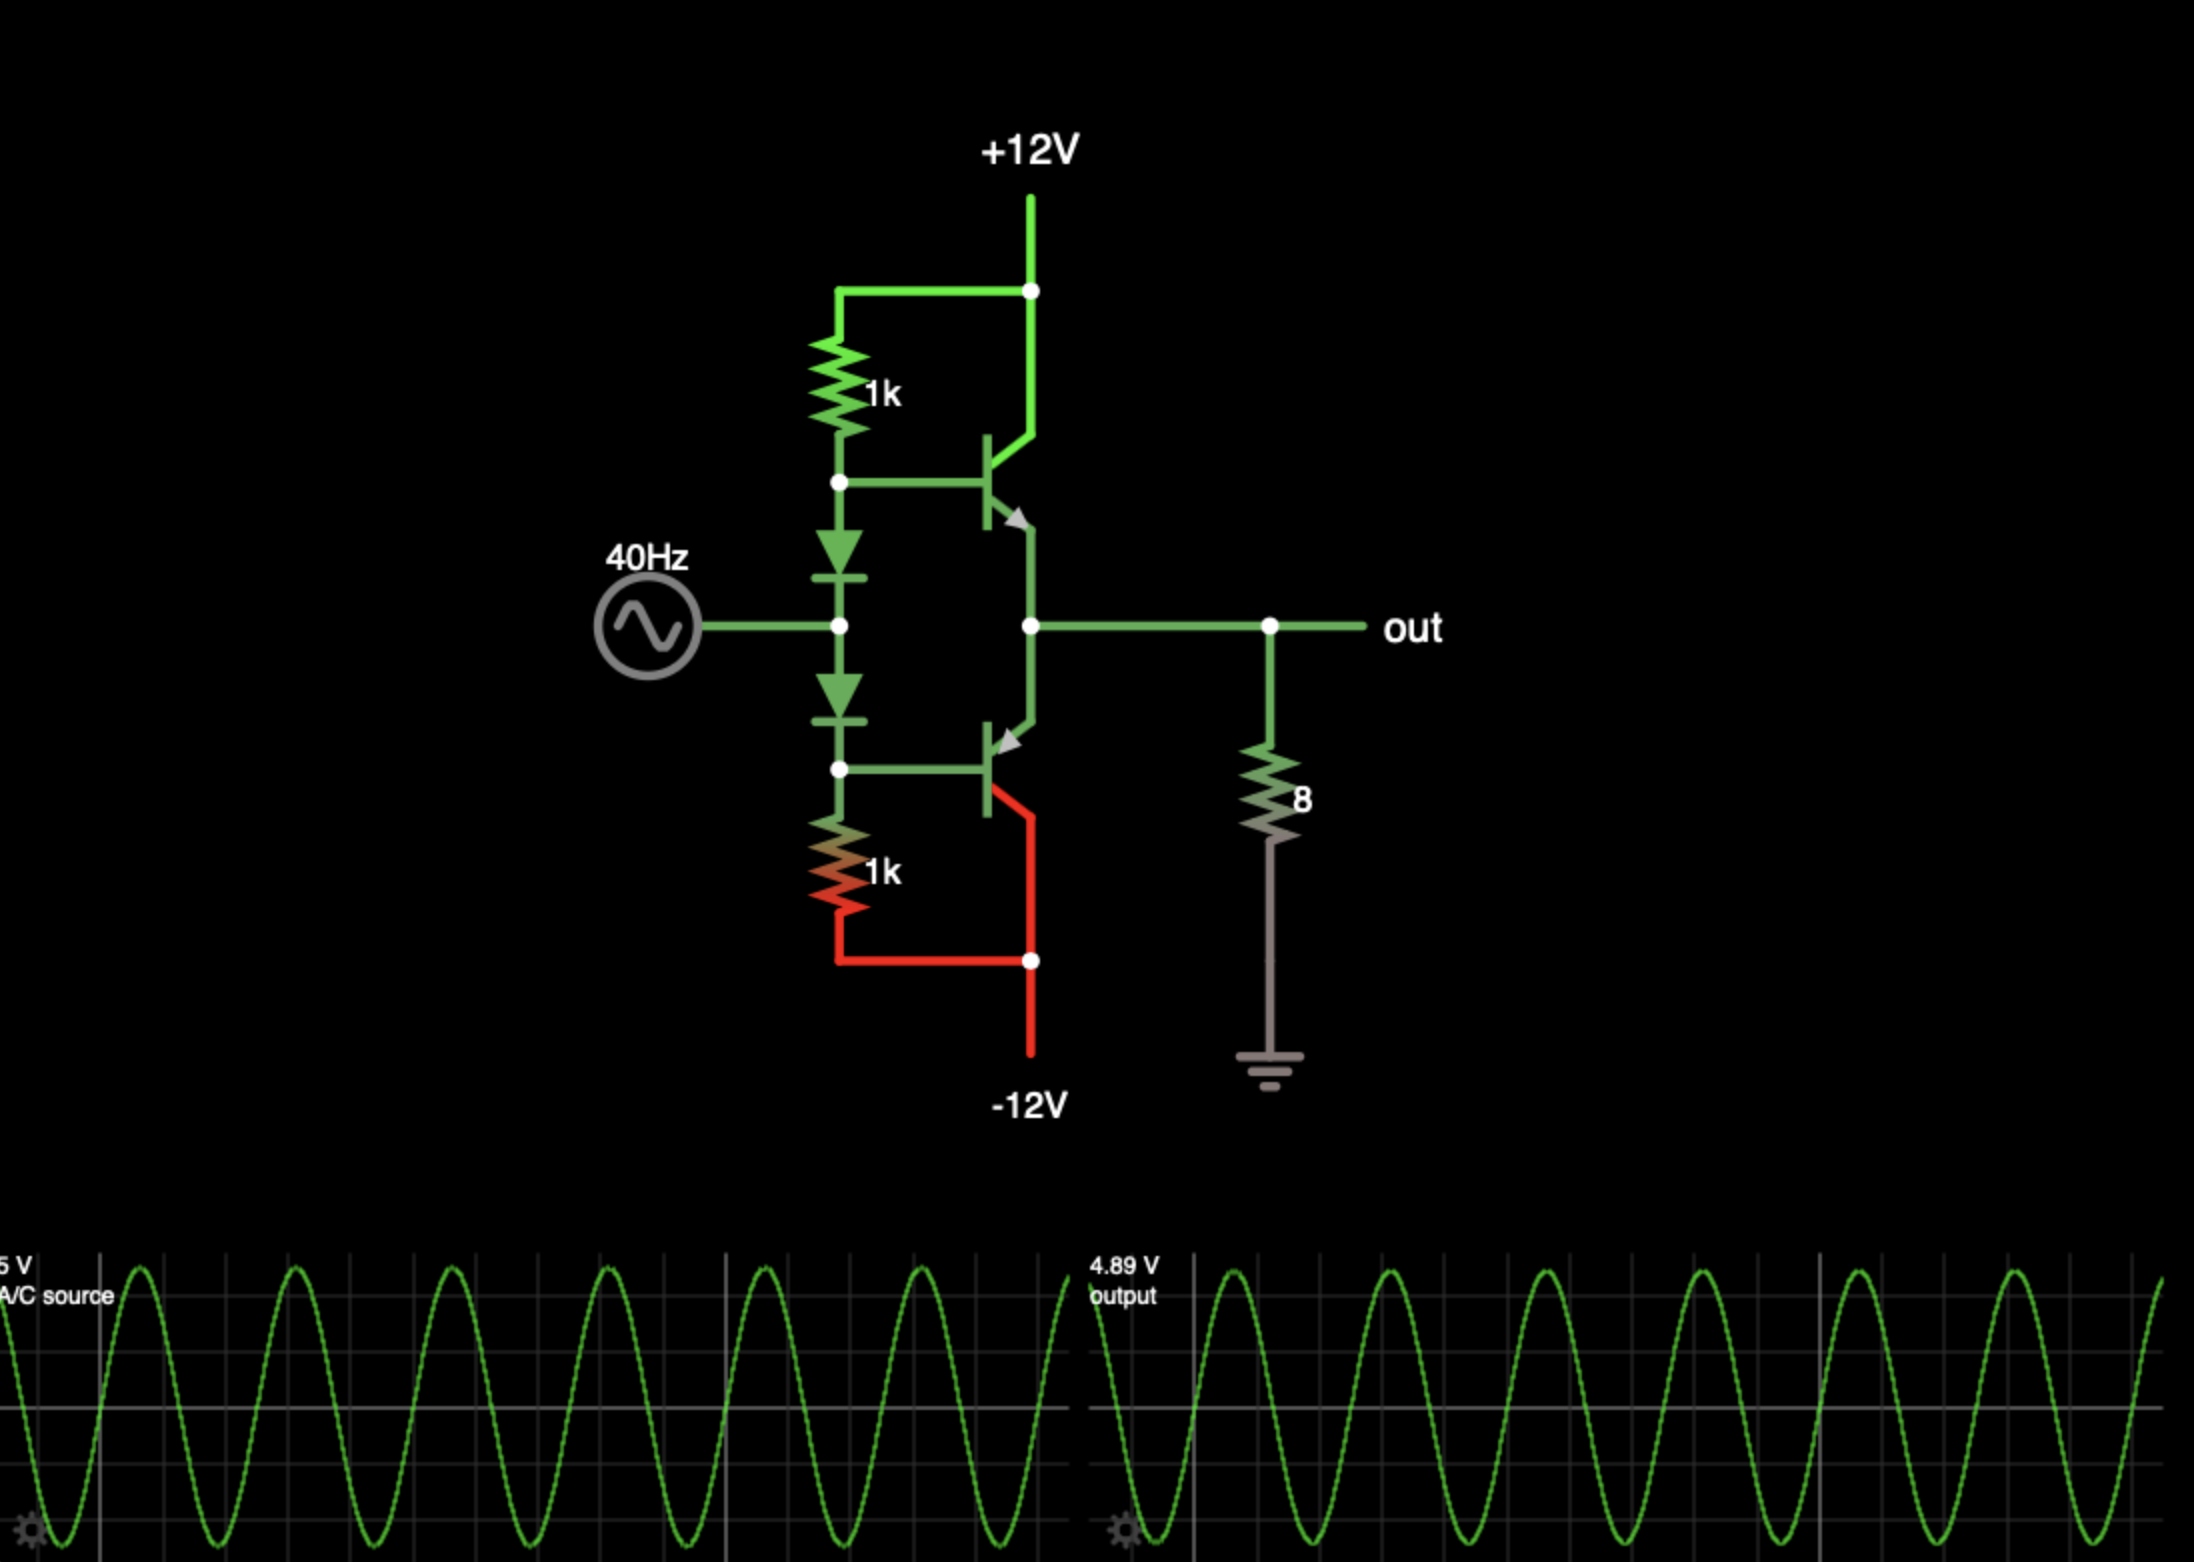
\includegraphics[width=13cm,height=13cm,keepaspectratio]{imagens/cicloPos.png}
        \caption{Circuito \emph{push-pull} no semi-ciclo positivo da fonte de tensão.}
        \label{fig:push-pull-pos}
    \end{figure}


\end{document}

